%
% problemstellung.tex -- Beispiel-File für die Beschreibung des Problems
%
% (c) 2020 Prof Dr Andreas Müller, Hochschule Rapperswil
%
\section{Beispiele von ähnlichen Funktionen
\label{logistic:section:beispiele}}
\rhead{Beispiele von ähnlichen Funktionen}
\subsection{Mandelbrotmenge}
In Kapitel \ref{logistic:section:analyse} 
haben wir bereits gesehen, 
dass das Bifurkationsdiagramm der logistischen Gleichung
ein Fraktal ist. 
Eines der bekanntesten Fraktale ist die Mandelbrotmenge,
deren Gleichung der logistischen Gleichung sehr ähnlich ist. 
Die Gleichung der Mandelbrotmenge lautet
\begin{equation}
    z_{n+1} = z_n^2 + c
    \label{eq:mandelbrot}
\end{equation}
wobei $z_n$ und $c$ komplexe Zahlen sind und 
der Einfachkeit halber $z_0 = 0$ gesetzt werden kann.
Zum Vergleich, die logistische Gleichung hat ausmultipliziert
die Form $x_{n+1} = -\lambda x_n^2 +\lambda x_n$. 
Wie bei der logistischen Gleichung gibt es auch
bei der Gleichung der Mandelbrotmenge wieder bestimmte
Werte von $c$, bei der $z_n$ entweder 
divergiert, 
konvergiert, 
oszilliert 
oder in chaotisches Verhalten ausbricht. 
Jeder Wert von $c$, für den $z_n$ nicht 
divergiert, ist Teil der Mandelbrotmenge. 
Nun können wir, ähnlich wie schon beim 
Bifurkationendiagramm der logistischen Gleichung, auf der
komplexen Ebene für jeden Wert von $c$ das Verhalten
der Gleichung der Mandelbrotmenge darstellen. 
Dazu färben wir den Bereich, in dem $z_n$ 
nicht divergiert, rot ein.
Damit sehen wir auf Abbildung \ref{fig:mandel_2d}
die Mandelbrotmenge. 
\begin{figure}
    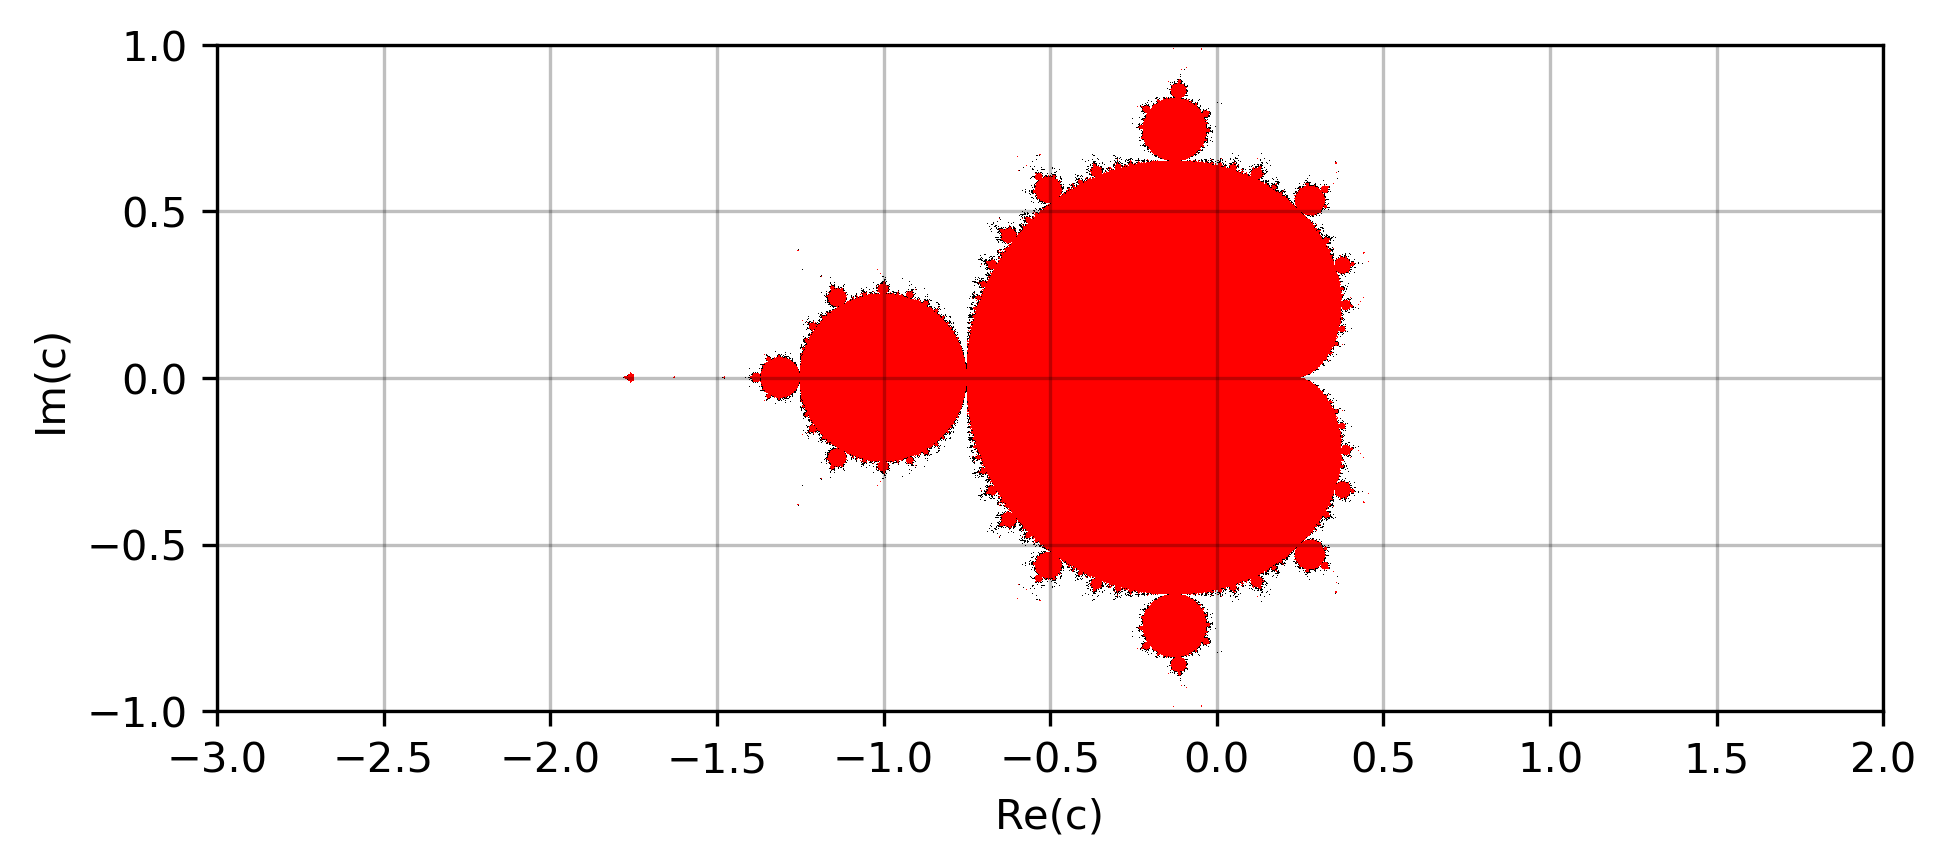
\includegraphics[width=\linewidth]{papers/logistic/figures/mandel.png}
    \caption{Mandelbrotmenge}
    \label{fig:mandel_2d}
\end{figure}
Auf dieser zweidimensionalen Darstellung ist jedoch nicht zu sehen, 
welche Werte $z_n$ annimmt.
Darum nehmen wir jetzt die dritte Dimension zur Hilfe um,
wie schon beim Bifurkationendiagramm der logistischen Gleichung,
auf der vertikalen Achse darzustellen, 
auf welchem Wert sich der Betrag von $z_n$ schlussendlich einpendelt.
Oder eben auch nicht, wenn es oszilliert oder sogar
chaotisch wird. 
Das Ergebnis davon ist auf Abbildung 
\ref{fig:mandel_3d}
zu sehen. 
Auf der reellen Achse ist deutlich ein Gebilde zu sehen,
welches dem Bifurkationsdiagramm der logistischen
Gleichung sehr ähnlich sieht. 
Ebenfalls zu sehen ist, dass die kreisförmigen
``Platformen'' sich regelmässig verdoppeln, weil
$z_n$ zwischen immer mehr Werten hin und her oszilliert.
\begin{figure}
    
\includegraphics[width=\linewidth]{papers/logistic/figures/mandel_3d.png}
    \caption{Bifurkationsdiagramm der Mandelbrotmenge}
    \label{fig:mandel_3d}
\end{figure}
\subsection{Universelle Eigenschaft}
Damit kommen wir auch schon zum nächsten Punkt. 
Dieses ganze Verhalten mit den Periodenverdoppelungen 
bis es schliesslich chaotisch wird und dann
immer wieder kurzen oszillierenden Fenstern im Chaos
ist keineswegs eine Eigenschaft, 
die nur die logistische Gleichung besitzt.
Man findet dieses Verhalten auch beim Iterieren 
von vielen anderen nichtlinearen Funktionen. 
Ein typisches Merkmal, 
an dem man Funktionen erkennt
die diese Eigenschaften aufweisen, 
sind ``Hügel'' im Funktionsplot.
Als Beispiel dazu sind in Abbildung \ref{fig:universal} links
die beiden Funktionen
$\lambda \cdot \cos(x)$
und
$\lambda \cdot (2 - \cosh(x))$
abgebildet.
Beide Funktionen haben, wie auch schon die Funktion
der logistischen Gleichung, einen Hügel. 
Rechts sind die Bifurkationsdiagramme dieser beiden
Funktionen abgebildet. 
Die Ähnlichkeiten zum Bifurkationsdiagramm der logistischen
Gleichung sind deutlich sichtbar. 
Abschliessend können wir so aus dieser Erkenntnis direkt 
noch etwas für die weitere Numerik mitnehmen.
Denn gerade in der Numerik bauen viele Verfahren
auf iterativen Algorithmen auf. 
Deswegen schadet es sicherlich nicht,
wenn man sich bewusst ist, dass beim Iterieren von
scheinbar einfachen Funktionen so ein ``wildes'' 
Verhalten enstehen kann. 
\begin{figure}
    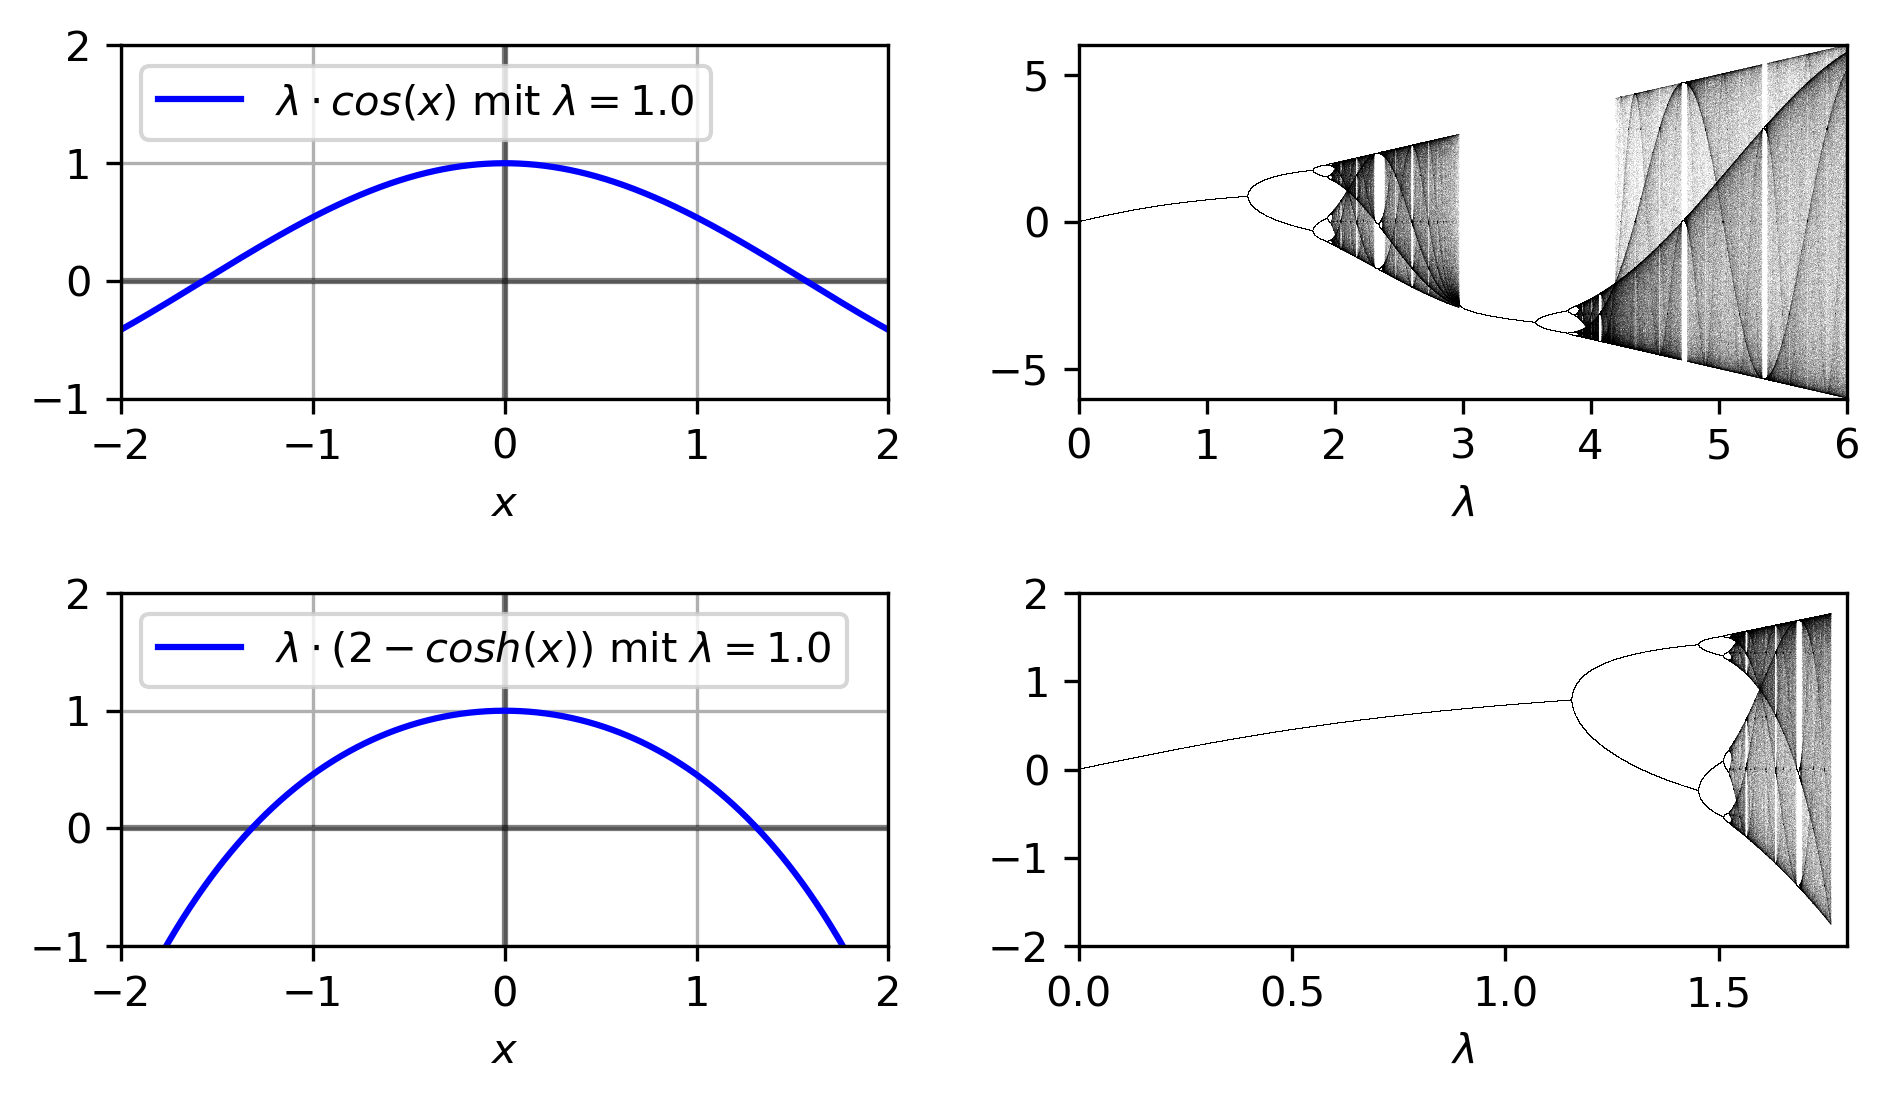
\includegraphics[width=\linewidth]{papers/logistic/figures/universal.png}
    \caption{
        Bifurkationsdiagramme von 
        $\lambda \cdot \cos(x)$
        und
        $\lambda \cdot (2 - \cosh(x))$.
    }
    \label{fig:universal}
\end{figure}
